\documentclass[a4paper,12pt]{article}

% --- Tiếng Việt + mã UTF-8 ---
\usepackage[utf8]{inputenc}
\usepackage[T5]{fontenc}
\usepackage[vietnamese]{babel}

% --- Bố cục trang ---
\usepackage{geometry}
\geometry{top=2.5cm, bottom=2.5cm, left=3cm, right=2cm}

% --- Toán ---
\usepackage{amsmath}
\usepackage{amssymb}

% --- Hình ảnh ---
\usepackage{graphicx}
\graphicspath{{img/}}

% --- Khung viền bìa ---
\usepackage{tikz}
\usetikzlibrary{calc}

% --- Liên kết ---
\usepackage{hyperref}

\begin{document}

% ================= KHUNG VIỀN BÌA =================
\begin{tikzpicture}[remember picture, overlay]
  \draw[line width=1.2pt, color=blue!40!black]
    ($(current page.north west)+(1.1cm,-1.1cm)$)
    rectangle ($(current page.south east)+(-1.1cm,1.1cm)$);
  \draw[line width=0.5pt, color=blue!40!black]
    ($(current page.north west)+(1.35cm,-1.35cm)$)
    rectangle ($(current page.south east)+(-1.35cm,1.35cm)$);
\end{tikzpicture}

% ================= TRANG BÌA =================
\begin{center}
ỦY BAN NHÂN DÂN THÀNH PHỐ HỒ CHÍ MINH

TRƯỜNG ĐẠI HỌC SÀI GÒN

KHOA TOÁN -- ỨNG DỤNG


\includegraphics[width=4cm]{SGU-LOGO.png}

\textbf{BÀI TẬP 3: PERCEPTRON VÀ MẠNG NƠ-RON}

Môn: Học sâu (Deep Learning)

Họ và tên: Đinh Quang Minh

MSSV: 3123580024

Lớp: DDU1231

Ngành: Khoa học dữ liệu

Giảng viên hướng dẫn: TS. Đỗ Như Tài

Học kỳ I, năm học 2026

TP. Hồ Chí Minh, tháng 10 năm 2026
\end{center}

\newpage

% ================================================================
\section*{PHẦN I. PERCEPTRON}

\subsection*{Câu 1}

Đường thẳng đã cho là $x_2 = -1.5x_1 + 3$. Chuyển hết sang một vế ta được
$1.5x_1 + x_2 - 3 = 0$.

Một perceptron có dạng $y = \tau(w_1x_1 + w_2x_2 + b)$, với $\tau(s) = +1$ khi $s \ge 0$
và $-1$ khi $s < 0$. Đối chiếu với phương trình trên thì
\[ w_1 = 1.5,\quad w_2 = 1,\quad b = -3, \]
nên perceptron cần tìm là
\[ y = \tau(1.5x_1 + x_2 - 3). \]

\subsection*{Câu 2}

\textbf{a)} Nhìn sơ đồ ta thấy trọng số nối vào nơ-ron gồm: từ bias là $-3$, từ $x_1$ là
$2.0$, từ $x_2$ là $1.0$. Vậy $w_1 = 2$, $w_2 = 1$, $b = -3$ và ranh giới quyết định là
\[ 2x_1 + x_2 - 3 = 0 \quad\Leftrightarrow\quad x_2 = -2x_1 + 3. \]

\textbf{b)} Lần lượt thay hai điểm vào $2x_1 + x_2 - 3$:

Với $\mathbf{x}^{(1)} = (-1, 0)$: $2(-1) + 0 - 3 = -5 < 0$, suy ra $y = -1$.

Với $\mathbf{x}^{(2)} = (2, 0)$: $2(2) + 0 - 3 = 1 \ge 0$, suy ra $y = +1$.

\textbf{c)} Đường thẳng trong hình cắt trục $x_1$ tại $2$ và trục $x_2$ tại $-1$, nên viết
theo đoạn chắn:
\[ \frac{x_1}{2} + \frac{x_2}{-1} = 1
   \;\Leftrightarrow\; x_1 - 2x_2 = 2
   \;\Leftrightarrow\; x_1 - 2x_2 - 2 = 0. \]
Đối chiếu với $w_1x_1 + w_2x_2 + b = 0$ ta có $w_1 = 1$, $w_2 = -2$, $b = -2$, tức
$y = f_g(x_1 - 2x_2 - 2)$.

\textbf{d)} Ở đây ngoài $x_1, x_2$ còn có đầu vào bias bằng $1$, nên cần chọn $w_1, w_2, b$.

\textit{Hàm AND.} Ta cần $(1,1)$ cho $+1$ còn ba điểm kia cho $-1$. Chọn $w_1 = w_2 = 1$,
$b = -1.5$:
\[
\begin{aligned}
(0,0)&:\ -1.5 < 0 \to -1, &\qquad (1,0)&:\ -0.5 < 0 \to -1,\\
(0,1)&:\ -0.5 < 0 \to -1, &\qquad (1,1)&:\ 0.5 \ge 0 \to +1.
\end{aligned}
\]
Vậy $y = \operatorname{sign}(x_1 + x_2 - 1.5)$.

\textit{Hàm OR.} Chỉ $(0,0)$ cho $-1$. Chọn $w_1 = w_2 = 1$, $b = -0.5$:
\[
\begin{aligned}
(0,0)&:\ -0.5 < 0 \to -1, &\qquad (1,0)&:\ 0.5 \ge 0 \to +1,\\
(0,1)&:\ 0.5 \ge 0 \to +1, &\qquad (1,1)&:\ 1.5 \ge 0 \to +1.
\end{aligned}
\]
Vậy $y = \operatorname{sign}(x_1 + x_2 - 0.5)$.

\subsection*{Câu 3}

Tập huấn luyện gồm $a=(0,0)^T$ với $t=-1$, còn $b=(1,0)^T$, $c=(0,1)^T$, $d=(1,1)^T$
đều có $t=+1$. Hàm mất mát
$J(\mathbf{w},b) = \sum_{\mathbf{x}_i \in Y}(-t_i)(\mathbf{w}^T\mathbf{x}_i + b)$,
trong đó $Y$ là tập các mẫu bị phân lớp sai.

\textbf{a)} Vì $J$ là tổng tuyến tính theo $\mathbf{w}$ và $b$ nên
\[ \frac{\partial J}{\partial \mathbf{w}} = \sum_{\mathbf{x}_i \in Y}(-t_i)\mathbf{x}_i,
   \qquad
   \frac{\partial J}{\partial b} = \sum_{\mathbf{x}_i \in Y}(-t_i). \]
Theo gradient descent $\mathbf{w} \leftarrow \mathbf{w} - \rho\dfrac{\partial J}{\partial \mathbf{w}}$,
thay dấu thì được công thức cập nhật
\[ \mathbf{w} \leftarrow \mathbf{w} + \rho\sum_{\mathbf{x}_i \in Y} t_i\mathbf{x}_i,
   \qquad
   b \leftarrow b + \rho\sum_{\mathbf{x}_i \in Y} t_i. \]

\textbf{b)} Các bước chạy batch perceptron learning:
\begin{enumerate}
  \item Chọn $\mathbf{w}$, $b$ ban đầu và tốc độ học $\rho > 0$.
  \item Đặt $d\mathbf{w} = \mathbf{0}$, $db = 0$.
  \item Duyệt từng mẫu $(\mathbf{x}_i, t_i)$: tính $s = \mathbf{w}^T\mathbf{x}_i + b$.
        Nếu $t_is < 0$ (phân lớp sai) thì cộng dồn $d\mathbf{w} \mathrel{+}= t_i\mathbf{x}_i$
        và $db \mathrel{+}= t_i$.
  \item Nếu không còn mẫu sai thì dừng. Ngược lại cập nhật
        $\mathbf{w} \mathrel{+}= \rho\,d\mathbf{w}$, $b \mathrel{+}= \rho\,db$ rồi quay lại bước 2.
\end{enumerate}

\textbf{c)} Đường thẳng trong hình là $x_2 = 0.5$, viết lại $0\cdot x_1 + 1\cdot x_2 - 0.5 = 0$.
Suy ra
\[ \mathbf{w}^{(0)} = (0,\ 1)^T, \qquad b^{(0)} = -0.5. \]

\textbf{d)} Chạy với $\rho = 0.4$. Ở vòng đầu, tính $s = \mathbf{w}^T\mathbf{x} + b$ cho từng mẫu:
\[ s_a = -0.5,\quad s_b = -0.5,\quad s_c = 0.5,\quad s_d = 0.5. \]
Xét dấu của $t_is$: mẫu $a$ có $(-1)(-0.5) = 0.5 > 0$ nên đúng, $b$ có $(+1)(-0.5) = -0.5 < 0$
nên sai, $c$ và $d$ đều đúng. Chỉ mẫu $b$ sai nên
\[ d\mathbf{w} = t_b\mathbf{x}_b = (1,0), \qquad db = t_b = 1, \]
\[ \mathbf{w}^{(1)} = (0,1) + 0.4(1,0) = (0.4,\ 1), \qquad
   b^{(1)} = -0.5 + 0.4 = -0.1. \]

Vòng hai, tính lại:
\[ s_a = -0.1,\quad s_b = 0.3,\quad s_c = 0.9,\quad s_d = 1.3. \]
Cả bốn mẫu đều cho $t_is > 0$, không còn mẫu sai nên thuật toán dừng.

Ranh giới tìm được là $0.4x_1 + x_2 - 0.1 = 0$, hay $x_2 = -0.4x_1 + 0.1$. Hình dưới so sánh
đường ban đầu (nét đứt) và đường sau khi học (nét liền):

\begin{center}
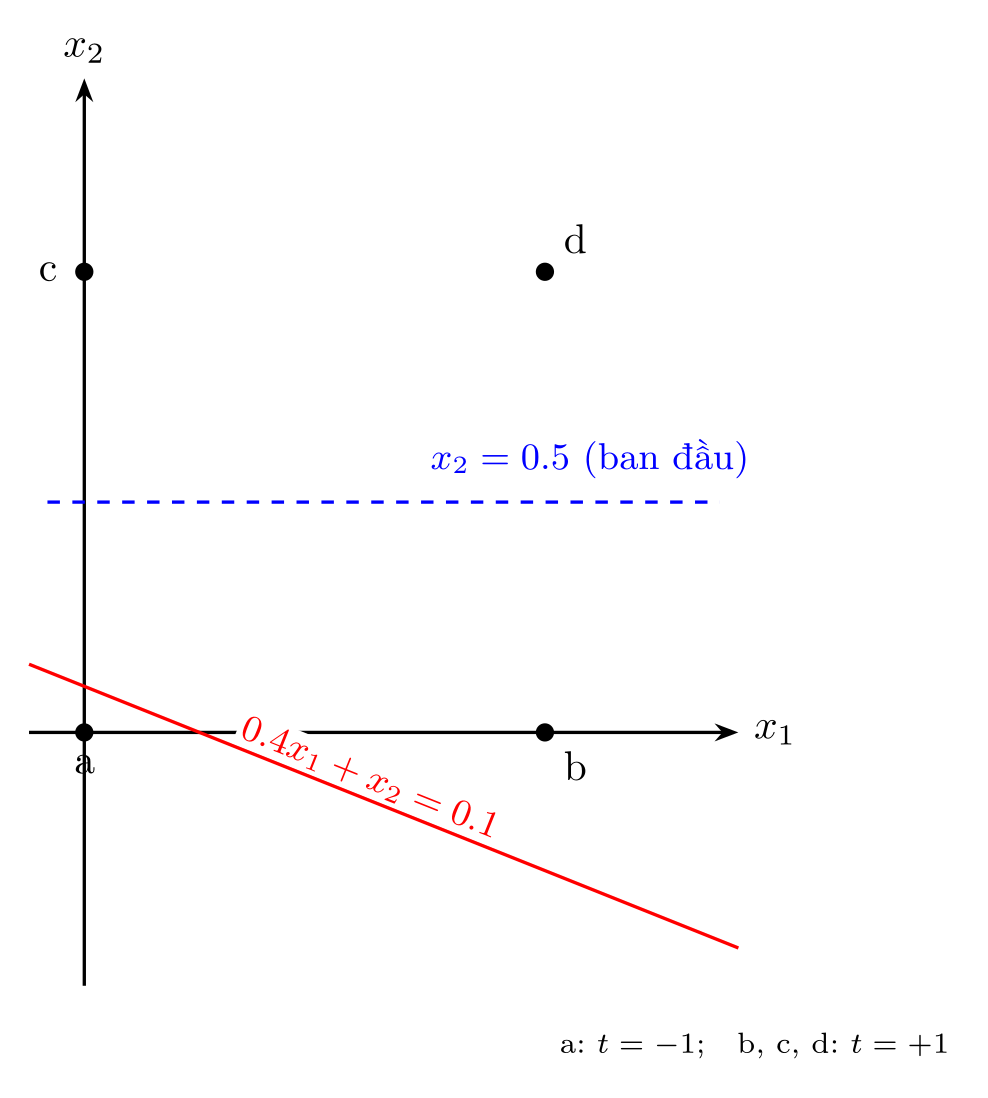
\includegraphics[width=0.66\textwidth]{p1_c3d.png}
\end{center}

\subsection*{Câu 4}

Với $w_1 = 0.3$, $w_2 = -0.2$, $\alpha = 0.2$ và ngưỡng $\theta = 0.4$ giữ cố định, đầu ra là
$Y = \text{Step}(x_1w_1 + x_2w_2 - \theta)$. Sai số $e = Y_d - Y$ và mỗi trọng số được cập nhật
theo $\Delta w_i = \alpha e x_i$, tức $w_i \leftarrow w_i + \Delta w_i$. Kết quả chạy từng mẫu:

\begin{center}
\begin{tabular}{|c|c|c|c|c|c|c|c|c|l|}
\hline
Epoch & $x_1$ & $x_2$ & $Y_d$ & $z$ & $Y$ & $e$ & $w_1$ & $w_2$ & Ghi chú \\
\hline
1 & 0 & 0 & 0 & $-0.40$ & 0 & 0 & 0.3 & $-0.2$ & giữ nguyên \\
1 & 0 & 1 & 0 & $-0.60$ & 0 & 0 & 0.3 & $-0.2$ & giữ nguyên \\
1 & 1 & 0 & 0 & $-0.10$ & 0 & 0 & 0.3 & $-0.2$ & giữ nguyên \\
1 & 1 & 1 & 1 & $-0.30$ & 0 & 1 & 0.5 & 0.0 & cập nhật \\
\hline
2 & 0 & 0 & 0 & $-0.40$ & 0 & 0 & 0.5 & 0.0 & giữ nguyên \\
2 & 0 & 1 & 0 & $-0.40$ & 0 & 0 & 0.5 & 0.0 & giữ nguyên \\
2 & 1 & 0 & 0 & $0.10$ & 1 & $-1$ & 0.3 & 0.0 & cập nhật \\
2 & 1 & 1 & 1 & $-0.10$ & 0 & 1 & 0.5 & 0.2 & cập nhật \\
\hline
3 & 0 & 0 & 0 & $-0.40$ & 0 & 0 & 0.5 & 0.2 & giữ nguyên \\
3 & 0 & 1 & 0 & $-0.20$ & 0 & 0 & 0.5 & 0.2 & giữ nguyên \\
3 & 1 & 0 & 0 & $0.10$ & 1 & $-1$ & 0.3 & 0.2 & cập nhật \\
3 & 1 & 1 & 1 & $0.10$ & 1 & 0 & 0.3 & 0.2 & giữ nguyên \\
\hline
4 & 0 & 0 & 0 & $-0.40$ & 0 & 0 & 0.3 & 0.2 & đúng \\
4 & 0 & 1 & 0 & $-0.20$ & 0 & 0 & 0.3 & 0.2 & đúng \\
4 & 1 & 0 & 0 & $-0.10$ & 0 & 0 & 0.3 & 0.2 & đúng \\
4 & 1 & 1 & 1 & $0.10$ & 1 & 0 & 0.3 & 0.2 & đúng \\
\hline
\end{tabular}
\end{center}

Sang epoch 4 thì cả bốn mẫu đều cho đầu ra đúng nên dừng lại. Trọng số cuối cùng là
$w_1 = 0.3$, $w_2 = 0.2$, $\theta = 0.4$, tương ứng đường phân cách
$0.3x_1 + 0.2x_2 = 0.4$.

% ================================================================
\newpage
\section*{PHẦN II. MẠNG NƠ-RON}

\subsection*{Câu 1}

\textbf{1.} Gọi $v_1, v_2, v_3$ là tổng có trọng số ở ba nơ-ron tầng ẩn. Mỗi nơ-ron nhận
ba đầu vào $(x_1, x_2, 1)$, thay các vector trọng số đã cho:
\[ v_1 = 2x_1 + 0x_2 + 1 = 2x_1 + 1, \]
\[ v_2 = 1x_1 + 2x_2 + 1 = x_1 + 2x_2 + 1, \]
\[ v_3 = 1x_1 + 3x_2 + 0 = x_1 + 3x_2. \]
Đầu ra tầng ẩn là $h_i = \varphi(v_i)$, nhận giá trị $0$ hoặc $1$. Nơ-ron đầu ra nhận
$h_1, h_2, h_3$ và bias $1$, nên
\[ v_4 = 2h_1 + 3h_2 + 1h_3 + 1\cdot 1 = 2h_1 + 3h_2 + h_3 + 1. \]

\textbf{2.} Vì $h_i \in \{0,1\}$ nên $2h_1 + 3h_2 + h_3 \ge 0$, do đó
\[ v_4 \ge 0 + 1 = 1 > 0. \]
Suy ra $y = \varphi(v_4) = 1$ với mọi $(x_1, x_2)$: mạng luôn kích hoạt.

\textbf{3.} Miền kích hoạt vì thế là toàn bộ mặt phẳng $(x_1, x_2)$. Ba đường ranh giới của
tầng ẩn (nơi $v_i = 0$) là
\[ x_1 = -0.5, \qquad x_1 + 2x_2 = -1, \qquad x_1 + 3x_2 = 0. \]

\begin{center}
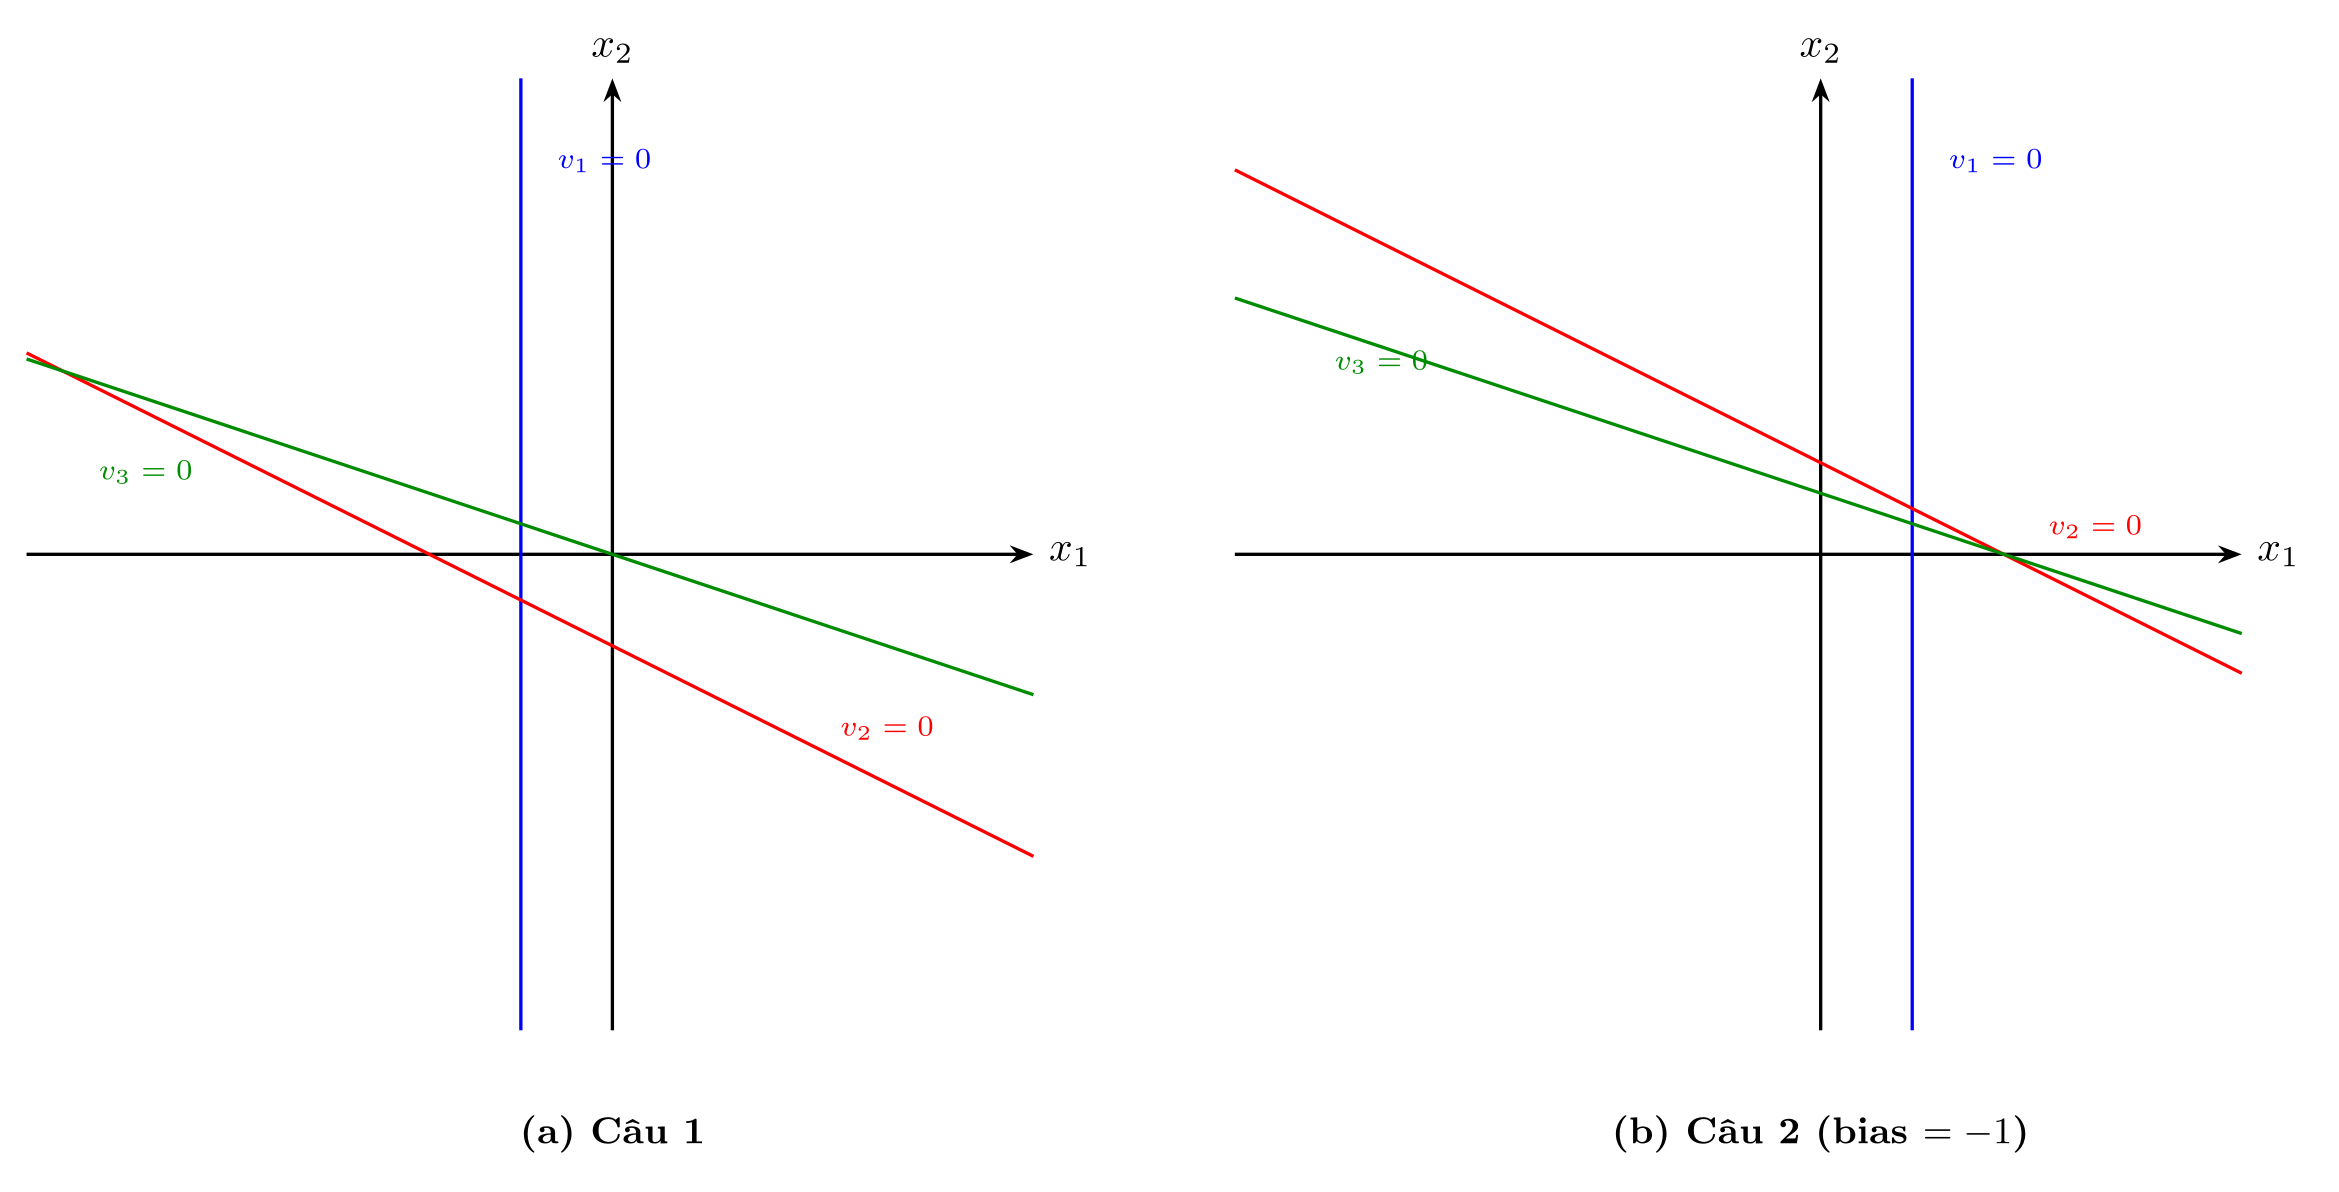
\includegraphics[width=0.98\textwidth]{p2_regions.png}
\end{center}

\textbf{4.} Ba đường trên chia mặt phẳng thành các vùng tương ứng với việc nơ-ron ẩn nào bật.
Tuy nhiên các trọng số nối vào nơ-ron ra đều dương và bias đầu ra bằng $+1$, nên dù không
nơ-ron ẩn nào bật thì $v_4$ vẫn bằng $1$ và đầu ra vẫn là $1$. Về hình học, toàn bộ mặt phẳng
nằm về phía dương của siêu phẳng quyết định.

\subsection*{Câu 2}

\textbf{1.} Đổi bias tầng ẩn từ $1$ thành $-1$, các trọng số còn lại giữ nguyên:
\[ w_1 = [2,\ 0,\ -1]^T, \qquad w_2 = [1,\ 2,\ -1]^T, \qquad w_3 = [1,\ 3,\ -1]^T, \]
và $w_4 = [2,\ 3,\ 1,\ 1]^T$ không đổi.

\textbf{2.} Tính lại tổng có trọng số ở tầng ẩn:
\[ v_1 = 2x_1 - 1, \qquad v_2 = x_1 + 2x_2 - 1, \qquad v_3 = x_1 + 3x_2 - 1, \]
với $h_i = \varphi(v_i)$ và $v_4 = 2h_1 + 3h_2 + h_3 + 1$ như cũ. Điều kiện để từng nơ-ron ẩn
bật là
\[ x_1 \ge 0.5, \qquad x_1 + 2x_2 \ge 1, \qquad x_1 + 3x_2 \ge 1. \]

\textbf{3.} Vẫn có $v_4 \ge 1 > 0$ nên đầu ra bằng $1$ trên toàn mặt phẳng, giống câu 1.

\textbf{4.} Hình (b) ở câu 1 vẽ ba đường ranh giới mới sau khi đổi bias.

\textbf{5.} So sánh ba đường ranh giới:

\begin{center}
\begin{tabular}{|c|c|c|}
\hline
Tầng ẩn & Bias $=1$ (câu 1) & Bias $=-1$ (câu 2) \\
\hline
$v_1 = 0$ & $x_1 = -0.5$ & $x_1 = 0.5$ \\
$v_2 = 0$ & $x_1 + 2x_2 = -1$ & $x_1 + 2x_2 = 1$ \\
$v_3 = 0$ & $x_1 + 3x_2 = 0$ & $x_1 + 3x_2 = 1$ \\
\hline
\end{tabular}
\end{center}

Các đường đều dịch về phía dương nên nơ-ron ẩn bật ít hơn trước. Tuy vậy miền kích hoạt của
cả mạng không thay đổi, vẫn là toàn mặt phẳng, vì bias $+1$ ở đầu ra đã bảo đảm $v_4 > 0$.
Như vậy bias tầng ẩn chỉ điều chỉnh ranh giới riêng của từng nơ-ron ẩn; muốn đổi ngưỡng
quyết định của cả mạng thì phải thay đổi bias (hoặc trọng số) ở tầng đầu ra.

\subsection*{Câu 3}

\textbf{1.} Đầu vào gồm $x_1$ là điểm trung bình (thang 4), $x_2$ là điểm hạnh kiểm và $x_3$
là điểm rèn luyện (cùng thang 10). Đầu ra $y \in \{0,1\}$, bằng $1$ nếu sinh viên đạt danh
hiệu. Trọng số tương ứng là $\mathbf{w} = (2,\ 1,\ 1)^T$.

\textbf{2.} Điểm danh hiệu là $D = 2x_1 + x_2 + x_3$ và điều kiện đạt là $D \ge 24$, nên
perceptron có dạng
\[ y = \varphi(2x_1 + x_2 + x_3 - 24). \]

\textbf{3.} Bias $b = -24$, hàm kích hoạt là hàm bước
$\varphi(v) = 1$ khi $v \ge 0$ và $0$ khi $v < 0$.

\textbf{4.} Sơ đồ mạng:

\begin{center}
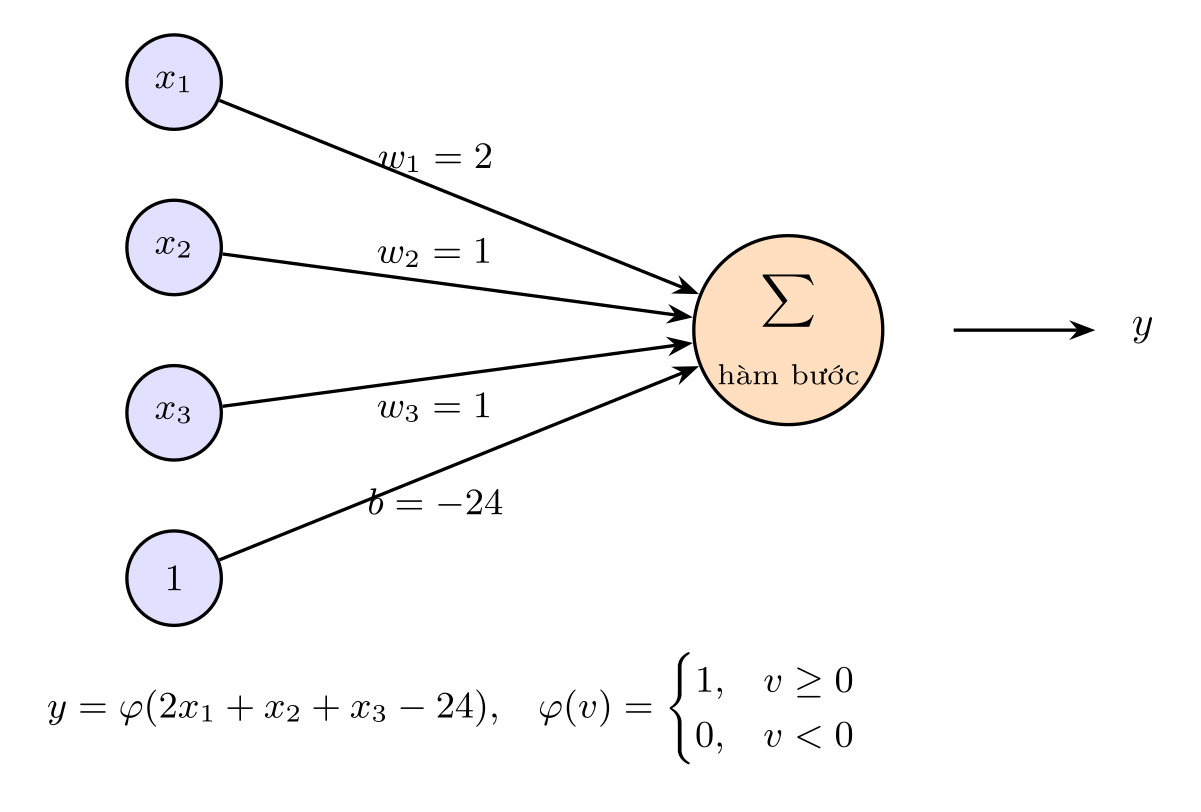
\includegraphics[width=0.76\textwidth]{p2_net.png}
\end{center}

\textbf{5.} Thay số cho ba sinh viên:
\begin{center}
\begin{tabular}{|c|c|c|c|c|c|}
\hline
SV & $x_1$ & $x_2$ & $x_3$ & $D = 2x_1 + x_2 + x_3$ & $y$ \\
\hline
SV1 & 3.5 & 9 & 9 & $7 + 9 + 9 = 25 \ge 24$ & 1 \\
SV2 & 3.0 & 8 & 9 & $6 + 8 + 9 = 23 < 24$ & 0 \\
SV3 & 4.0 & 10 & 10 & $8 + 10 + 10 = 28 \ge 24$ & 1 \\
\hline
\end{tabular}
\end{center}
Vậy SV1 và SV3 đạt danh hiệu, SV2 không đạt.

\textbf{6.} Điều kiện đạt danh hiệu là một bất đẳng thức tuyến tính theo ba biến
$2x_1 + x_2 + x_3 \ge 24$, tương ứng một siêu phẳng trong không gian 3 chiều. Bài toán phân
tách tuyến tính nên chỉ cần một nơ-ron với hàm bước là đủ, không phải dùng mạng nhiều tầng.

\subsection*{Câu 4}

\textbf{1.} Giữ nguyên các trọng số đầu vào, đổi bias thành $b$ thì tổng có trọng số là
\[ D = 2x_1 + x_2 + x_3 + b. \]

\textbf{2.} Sinh viên đạt danh hiệu khi $D \ge 0$, tức
\[ 2x_1 + x_2 + x_3 \ge -b. \]
Như vậy ngưỡng điểm danh hiệu là $T = -b$.

\textbf{3.} Chọn ba giá trị bias khác nhau:
\begin{center}
\begin{tabular}{|c|c|c|}
\hline
Bias $b$ & Ngưỡng $T = -b$ & Mức độ \\
\hline
$-20$ & 20 & dễ đạt \\
$-24$ & 24 & như đề bài \\
$-28$ & 28 & khó đạt \\
\hline
\end{tabular}
\end{center}

\textbf{4.} Áp dụng cho ba sinh viên ở câu 3:
\begin{center}
\begin{tabular}{|c|c|c|c|c|}
\hline
SV & $D$ & $b=-20$ & $b=-24$ & $b=-28$ \\
\hline
SV1 & 25 & đạt & đạt & không đạt \\
SV2 & 23 & đạt & không đạt & không đạt \\
SV3 & 28 & đạt & đạt & đạt \\
\hline
\end{tabular}
\end{center}

\textbf{5.} Khi bias tăng (bớt âm, ví dụ $-20$) thì ngưỡng $T = -b$ giảm xuống, tập sinh viên
được chọn rộng ra. Ngược lại khi bias âm hơn (ví dụ $-28$) thì ngưỡng tăng, tập được chọn
thu hẹp lại.

\textbf{6.} Bias đóng vai trò dịch chuyển ngưỡng quyết định: nó không làm đổi hướng của siêu
phẳng phân cách mà chỉ đẩy siêu phẳng đó ra xa hay gần gốc tọa độ. Nhờ vậy có thể chỉnh mức
"dễ" hay "khó" của bộ phân loại mà vẫn giữ nguyên trọng số của các đặc trưng.

\begin{center}
---o0o--- \\[0.3cm]
(Hết)
\end{center}

\end{document}
